\graphicspath{{06-Tracker/Figures/}}

\section{The Trackers}
\label{Sect:Tracker}

\subsection{Introduction}
MICE is equipped with two identical, high precision scintillating-fibre ("sciFi") trackers, described in [1]. Each tracker is placed in a superconducting solenoid designed to provide a uniform field over the tracking volume. One tracker, TKU, is upstream of the cooling cell, the other, TKD, downstream. Each tracker consists of five detector stations, labelled 1 to 5, with the stations placed varying distances apart to help resolve ambiguities. The trackers are placed symmetrically about the cooling cell, with station 1 the nearest to the cooling cell for both. Each station is formed of three planes of $350\mu m$ scintillating-fibres, orientated at 120 degrees to one another. Each plane consists of two layers. Thefibres in each plane butt up to each other and the two layers are offset with respect to each other by a fibre radius. A charge particle will then deposit energy in at least $350\mu m$ of scintillator, providing uniform response over the whole station face. The doublet layers are glued to a sheet of mylar and the fibres are adjacent groups of seven fibres form one read-out channel. The three views are referred to as U, V and W, with the order being identical for each station and the U fibres running vertically.
The light from the seven scintillating fibres passes into a single clear fibre, which takes it to a visible light photon counter (VLPC) which operate at 9k. The signal from the VLPCs is digitised using electronics developed by the D0 collaboration[2].


\subsection{Tracker Performance and Reconstruction}

\subsubsection{Low Level Analysis}
Low level analysis including digits, to spacepoints, 2 pages, Melissa U.
\begin{figure}[ht]
\begin{center}
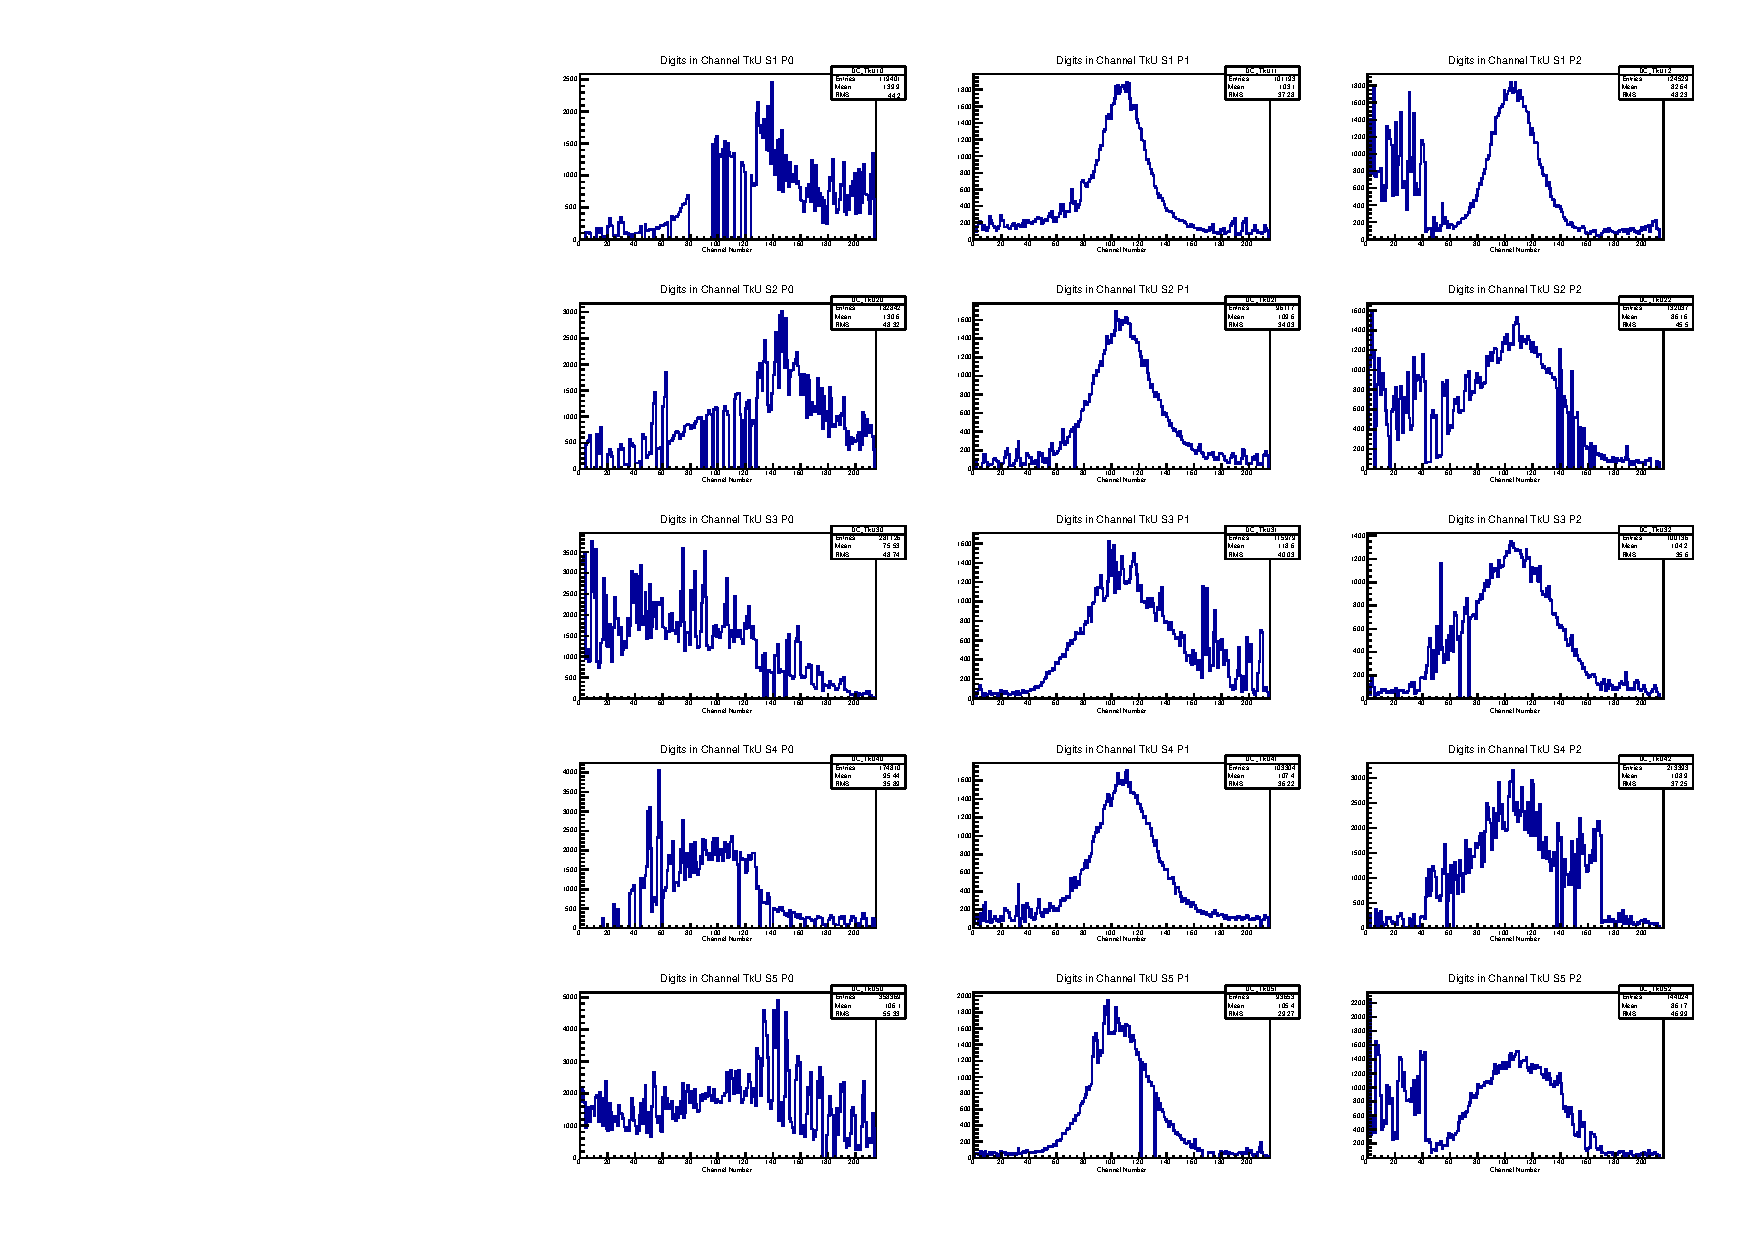
\includegraphics[width=\textwidth,keepaspectratio=true,]{Digits_Up.pdf}
\end{center}
\caption{}
\label{Figure:Digits_Up}
\end{figure}

\begin{figure}[ht]
\begin{center}
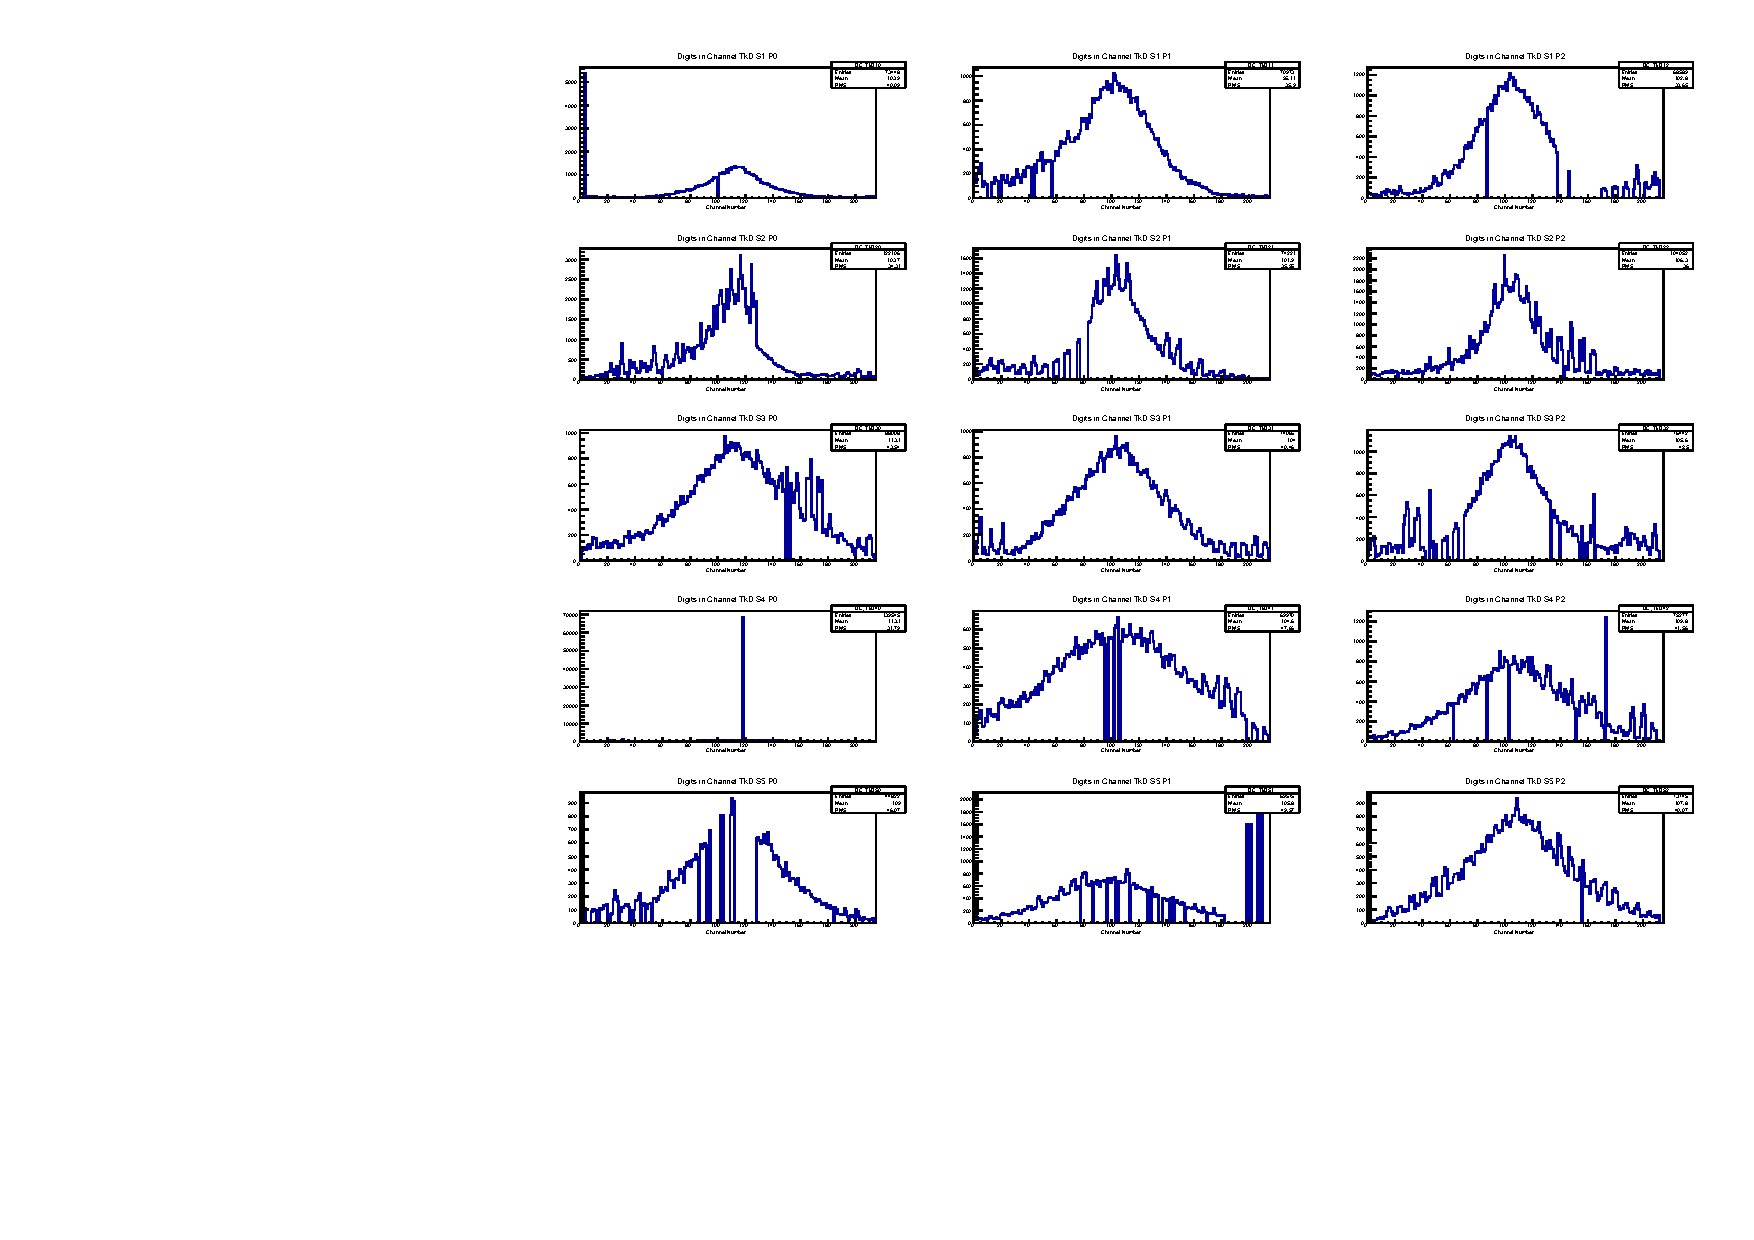
\includegraphics[width=\textwidth,keepaspectratio=true,]{Digits_Down.pdf}
\end{center}
\caption{}
\label{Figure:Digits_Down}
\end{figure}

\begin{figure}[!ht]
\begin{center}
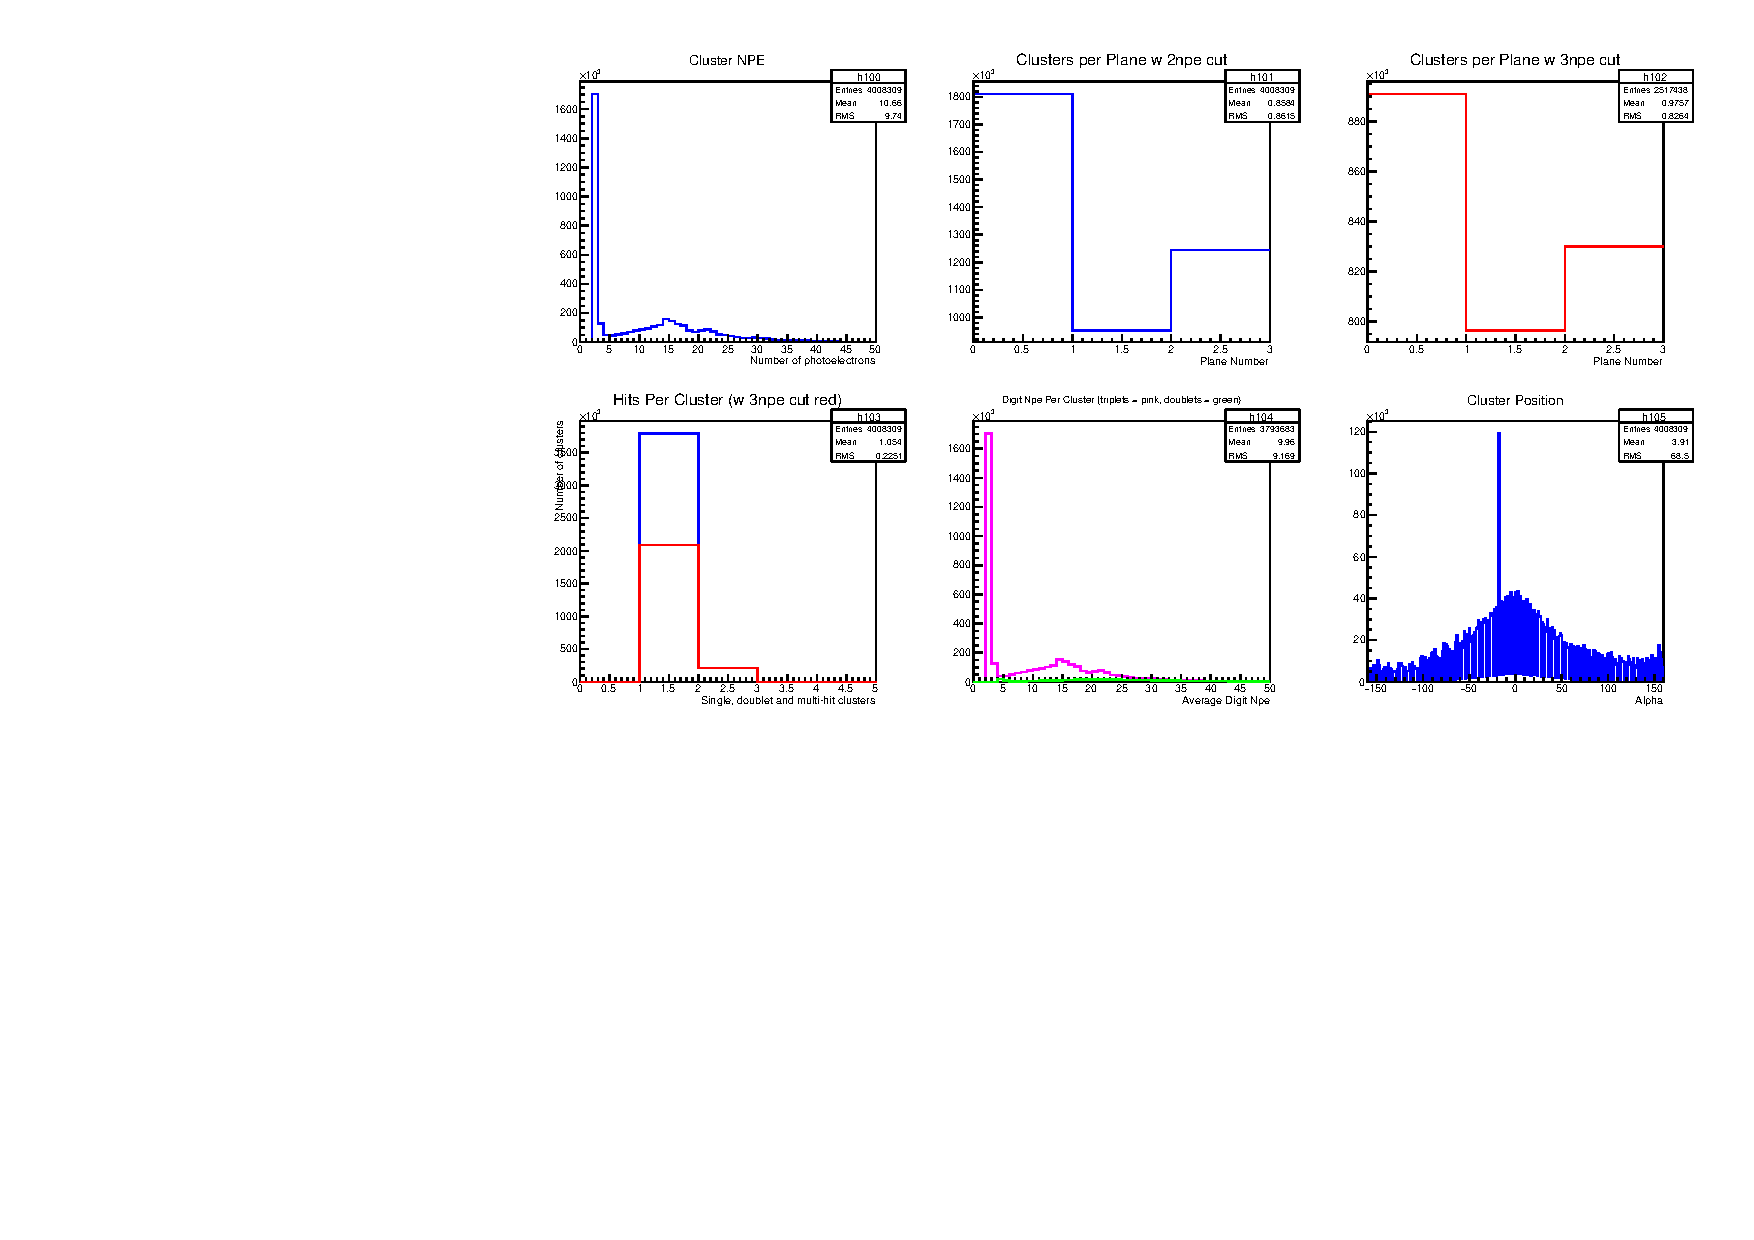
\includegraphics[width=\textwidth,keepaspectratio=true,]{Clusters.pdf}
\end{center}
\caption{}
\label{Figure:Clusters}
\end{figure}

\begin{figure}[!ht]
\begin{center}
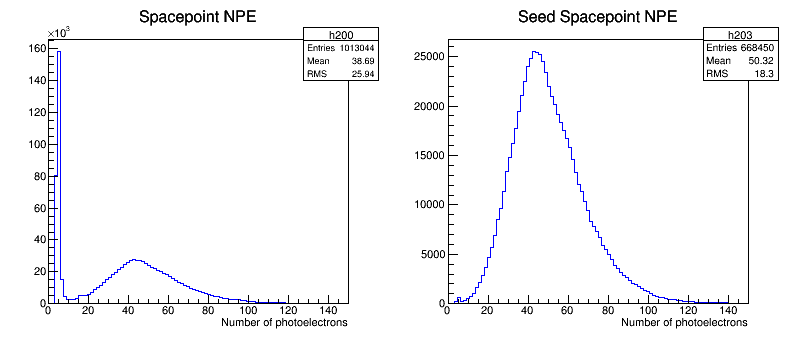
\includegraphics[width=\textwidth,keepaspectratio=true,]{SPSeeds10314.png}
\end{center}
\caption{[left] The NPE of each spacepoint in the US and DS trackers combined. [Right] only the NPE of those spacepoints which go on to make tracks in the US and DS trackers combined are shown.}
\label{Figure:SPSeeds_10314}
\end{figure}


\begin{figure}[ht]
	\centering
    \begin{tabular}{cc}
	    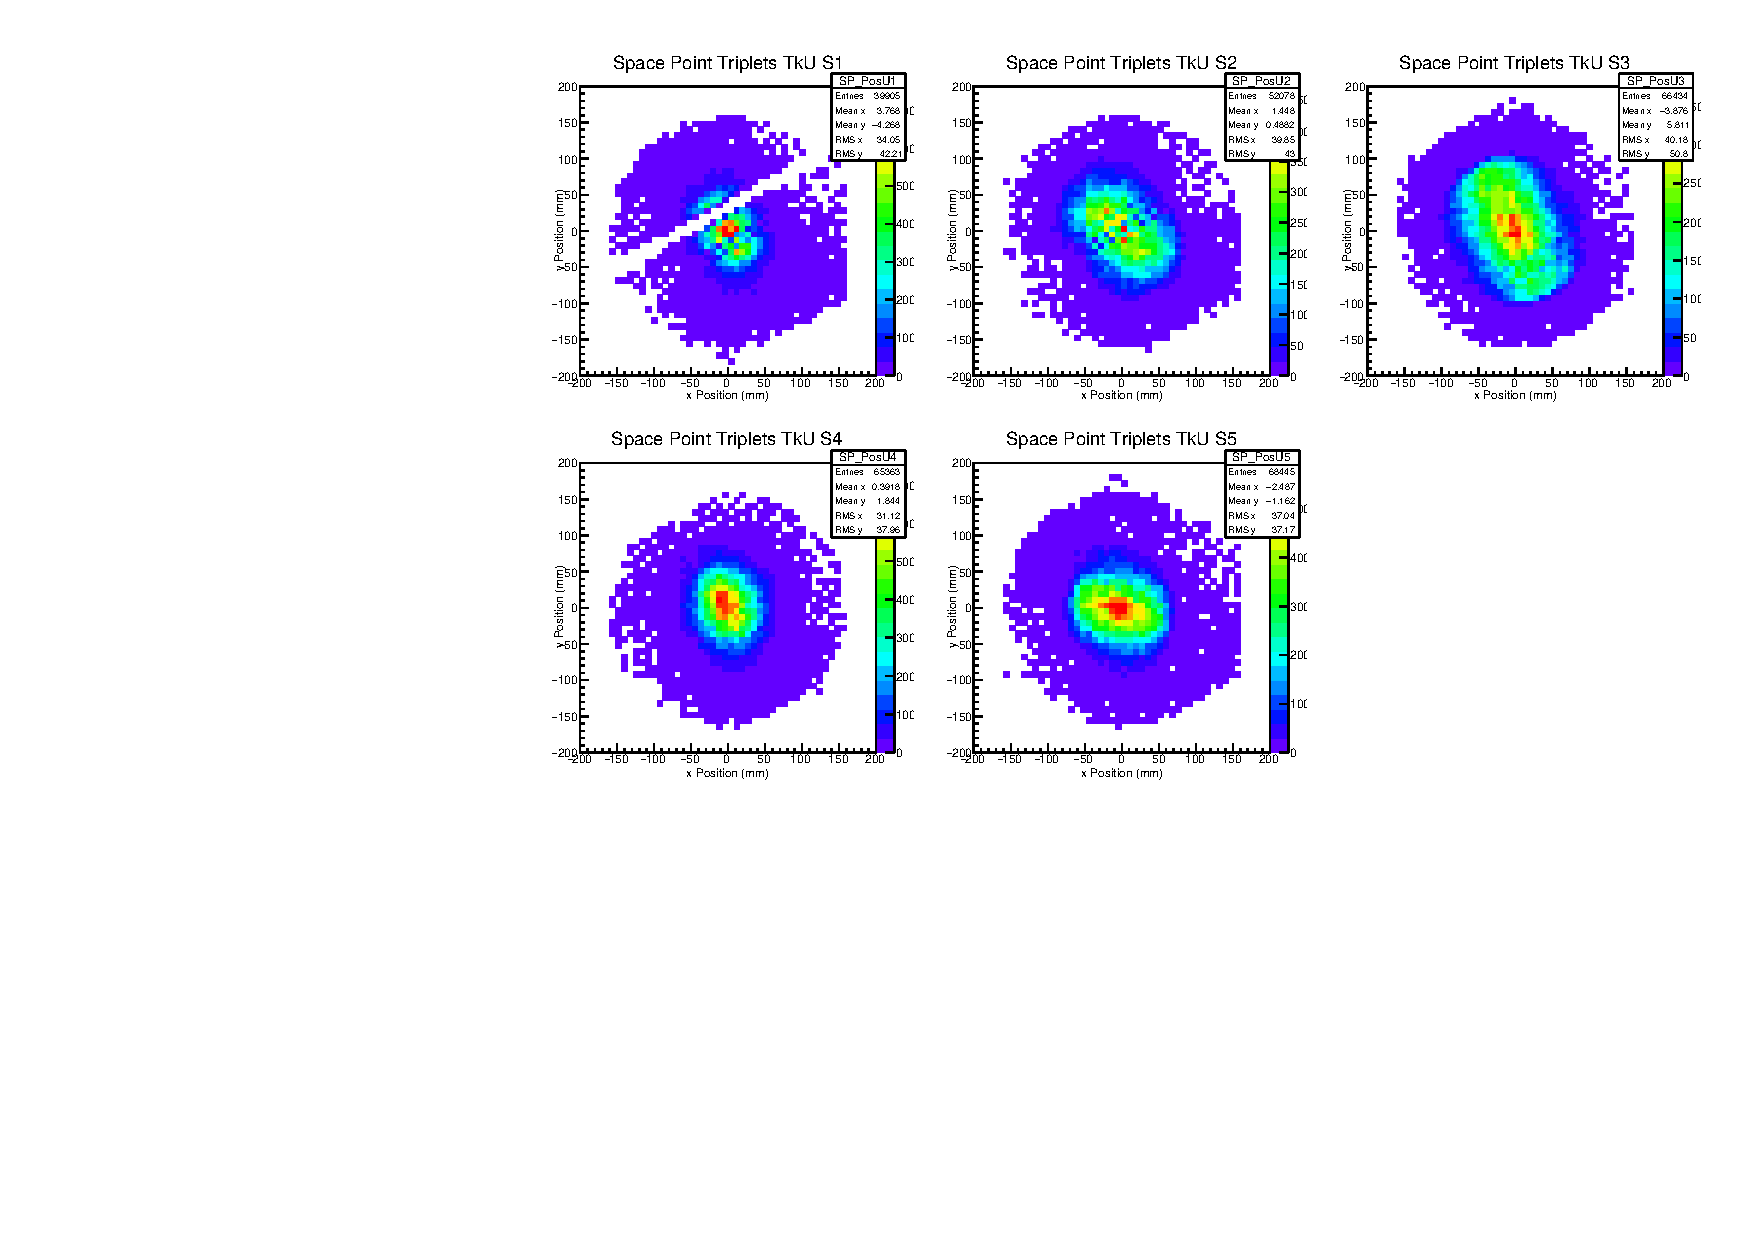
\includegraphics[width=0.5\textwidth]{Spacepoint_tripets_Up.pdf} &	
        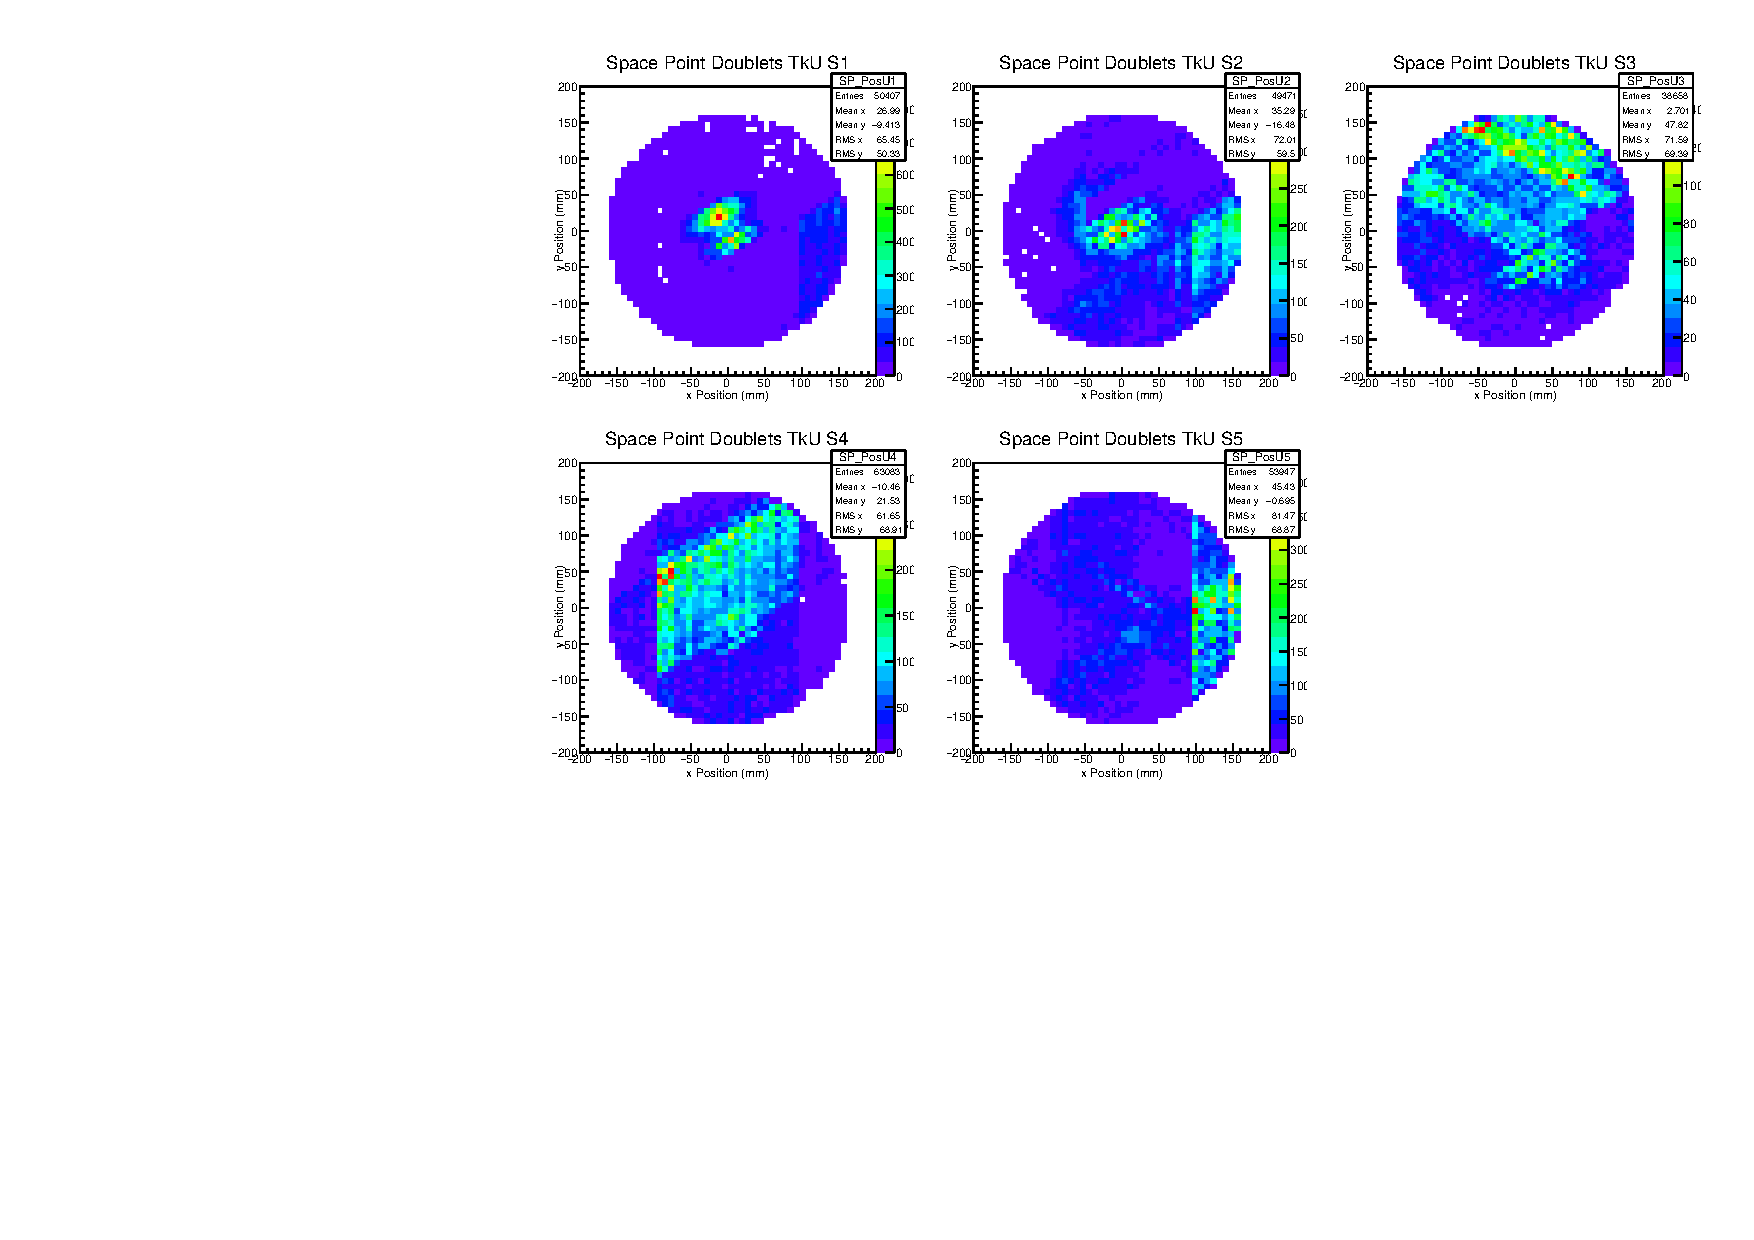
\includegraphics[width=0.5\textwidth]{Spacepoint_Doublets_Up.pdf} \\
    \end{tabular}
	\caption{\label{SP_US}}
\end{figure}

\begin{figure}[ht]
	\centering
    \begin{tabular}{cc}
	    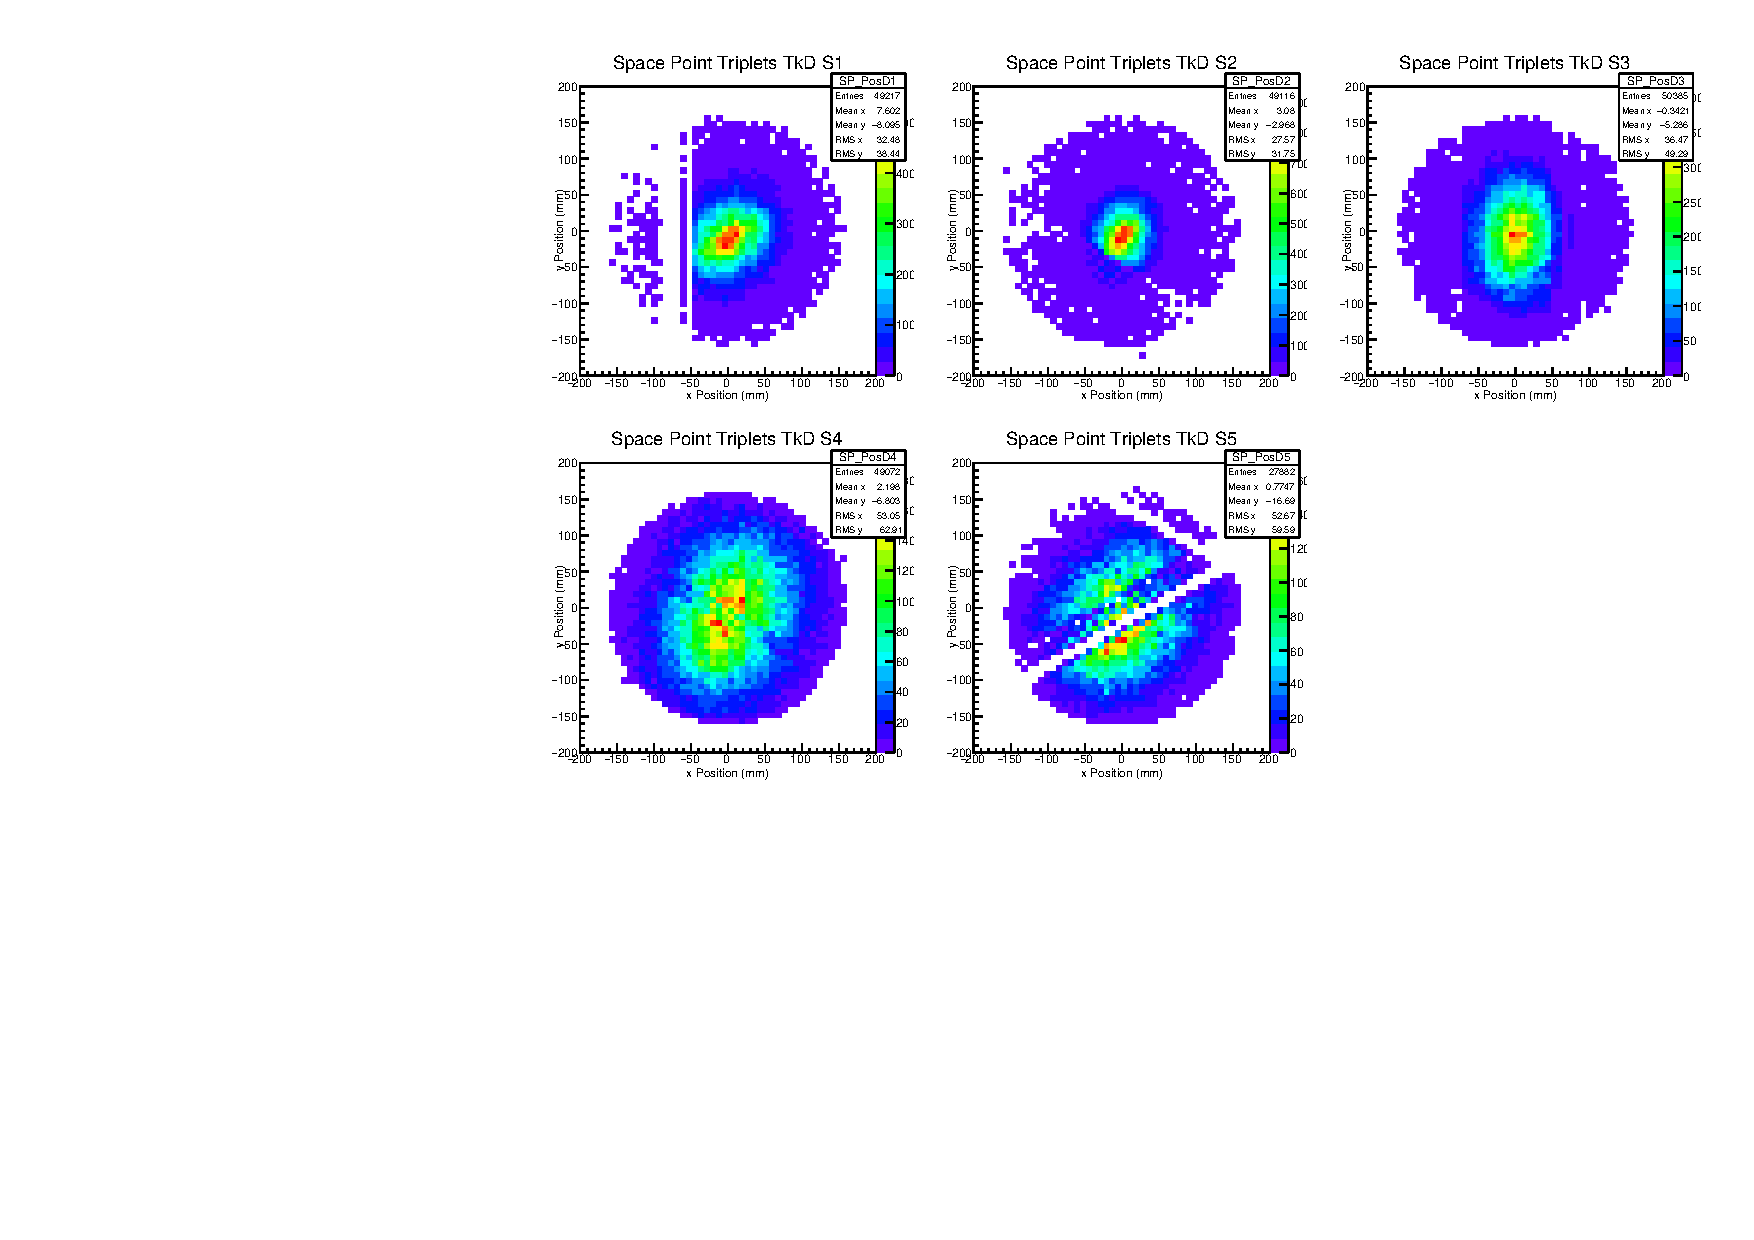
\includegraphics[width=0.5\textwidth]{Spacepoint_tripets_Down.pdf} &	
        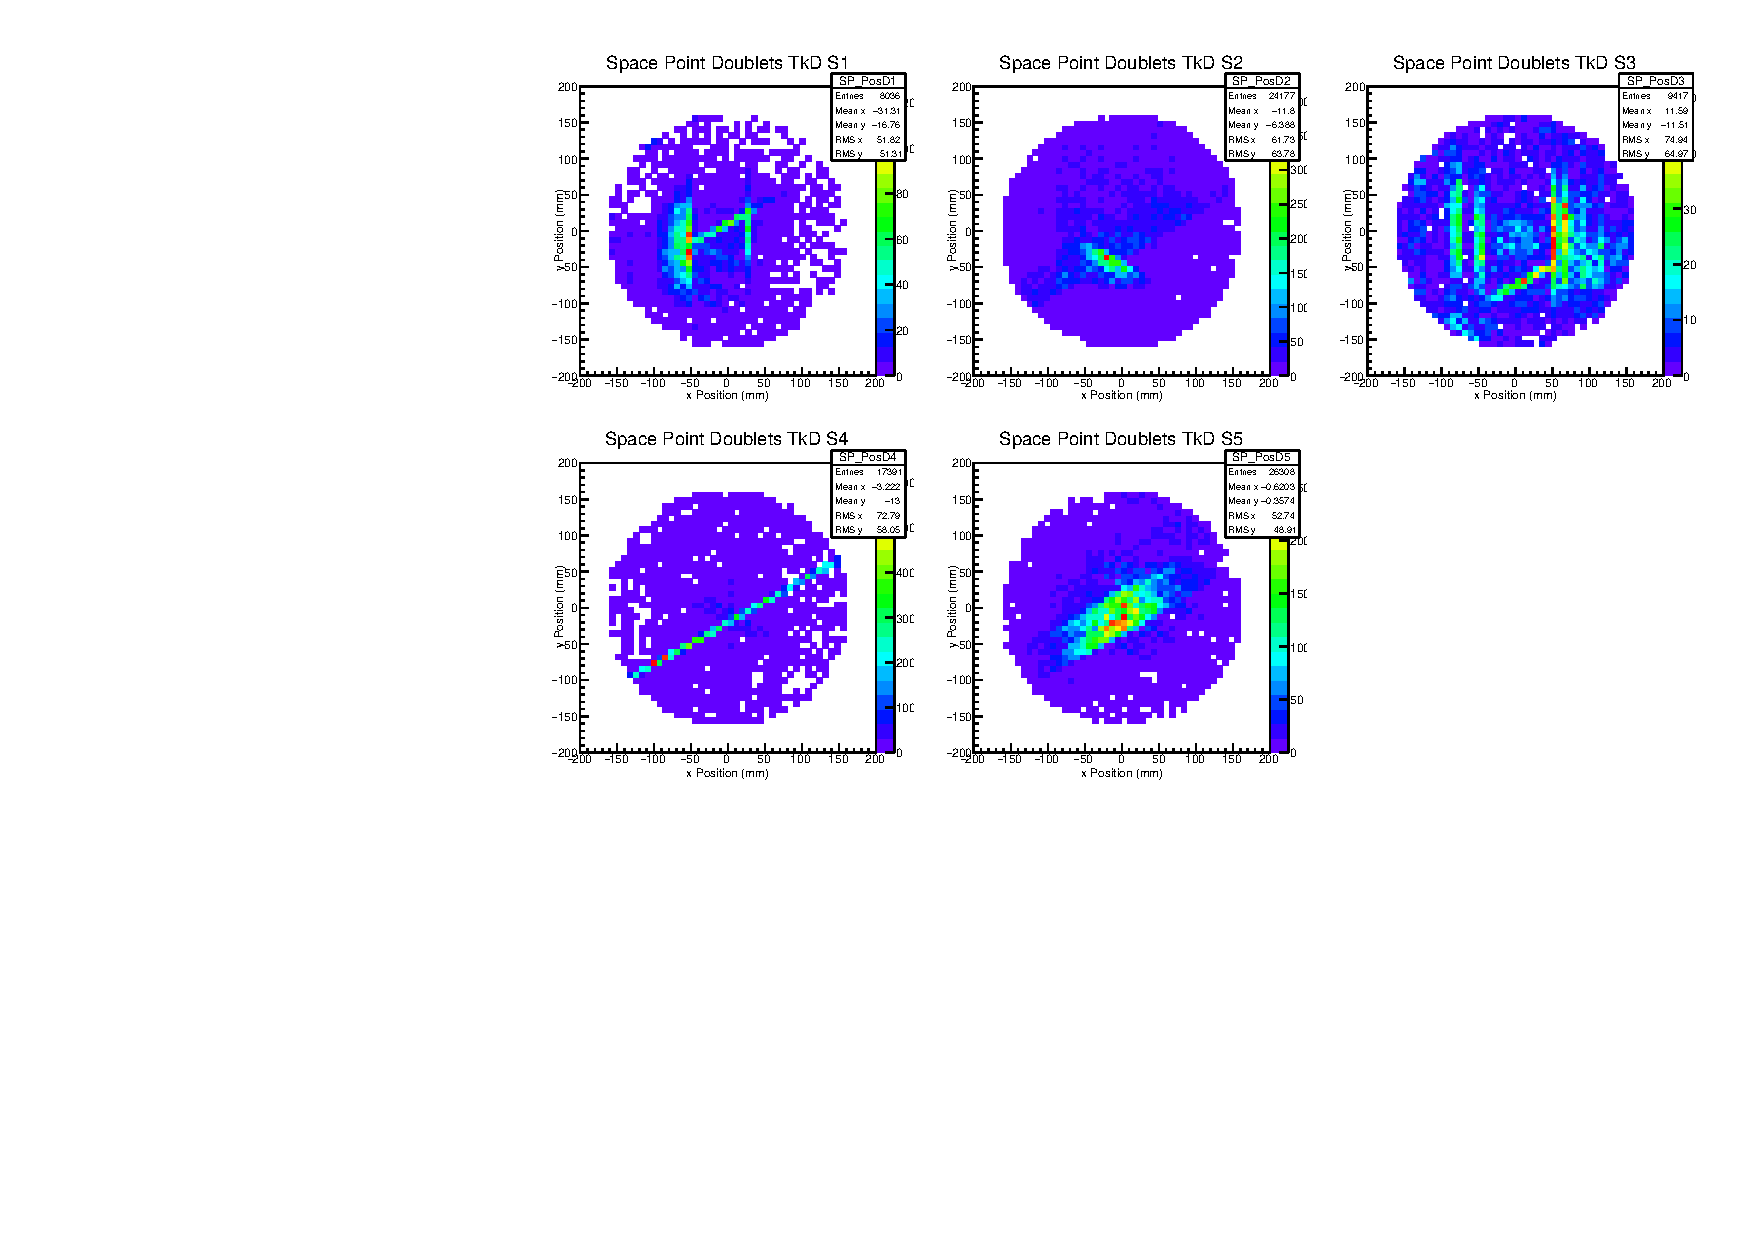
\includegraphics[width=0.5\textwidth]{Spacepoint_Doublets_Down.pdf} \\
    \end{tabular}
	\caption{\label{SP_DS}}
\end{figure}

\subsubsection{Noise}
Noise at electronics level discussion, 1/2 page, Chris H
and
Noise from data, 1/2 page, Chris H

\subsubsection{Track Finding Efficiency}
Track selection/Kalman, efficiency (from all data runs plotted by pt and if all equal just 10mm can be shown) resolution (from MC), reference MAUS and Tracker SW paper, 1 page, Chris H.

\subsubsection{Track Fit Predicted Performance}

Monte Carlo simulation used with realistic field and beam conditions in order to estimate the reconstruction performance. Run number 09964 was used, representing a typical data set used for the study of emittance evolution.

\begin{figure}[ht]
	\centering
    \begin{tabular}{cc}
	    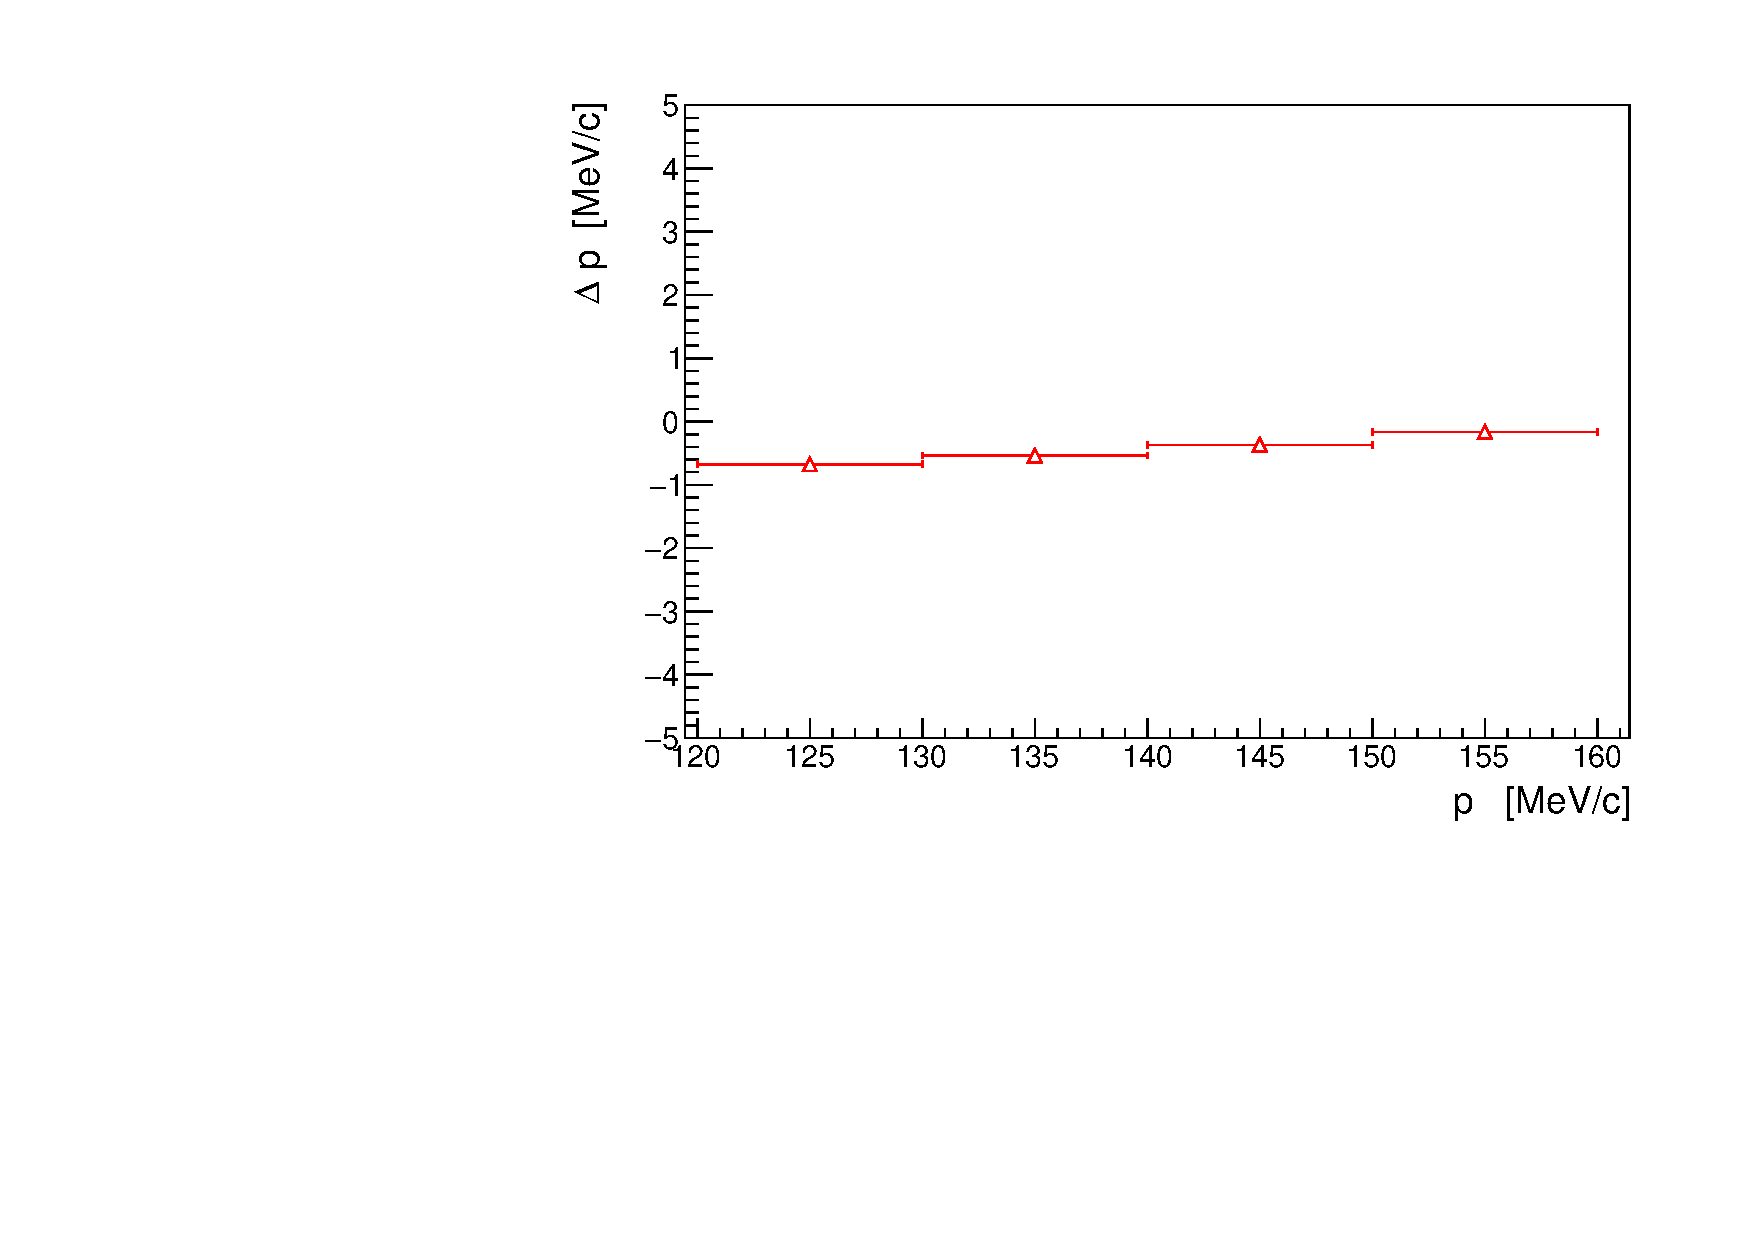
\includegraphics[width=0.5\textwidth]{upstream_p_bias_p.pdf} &	
        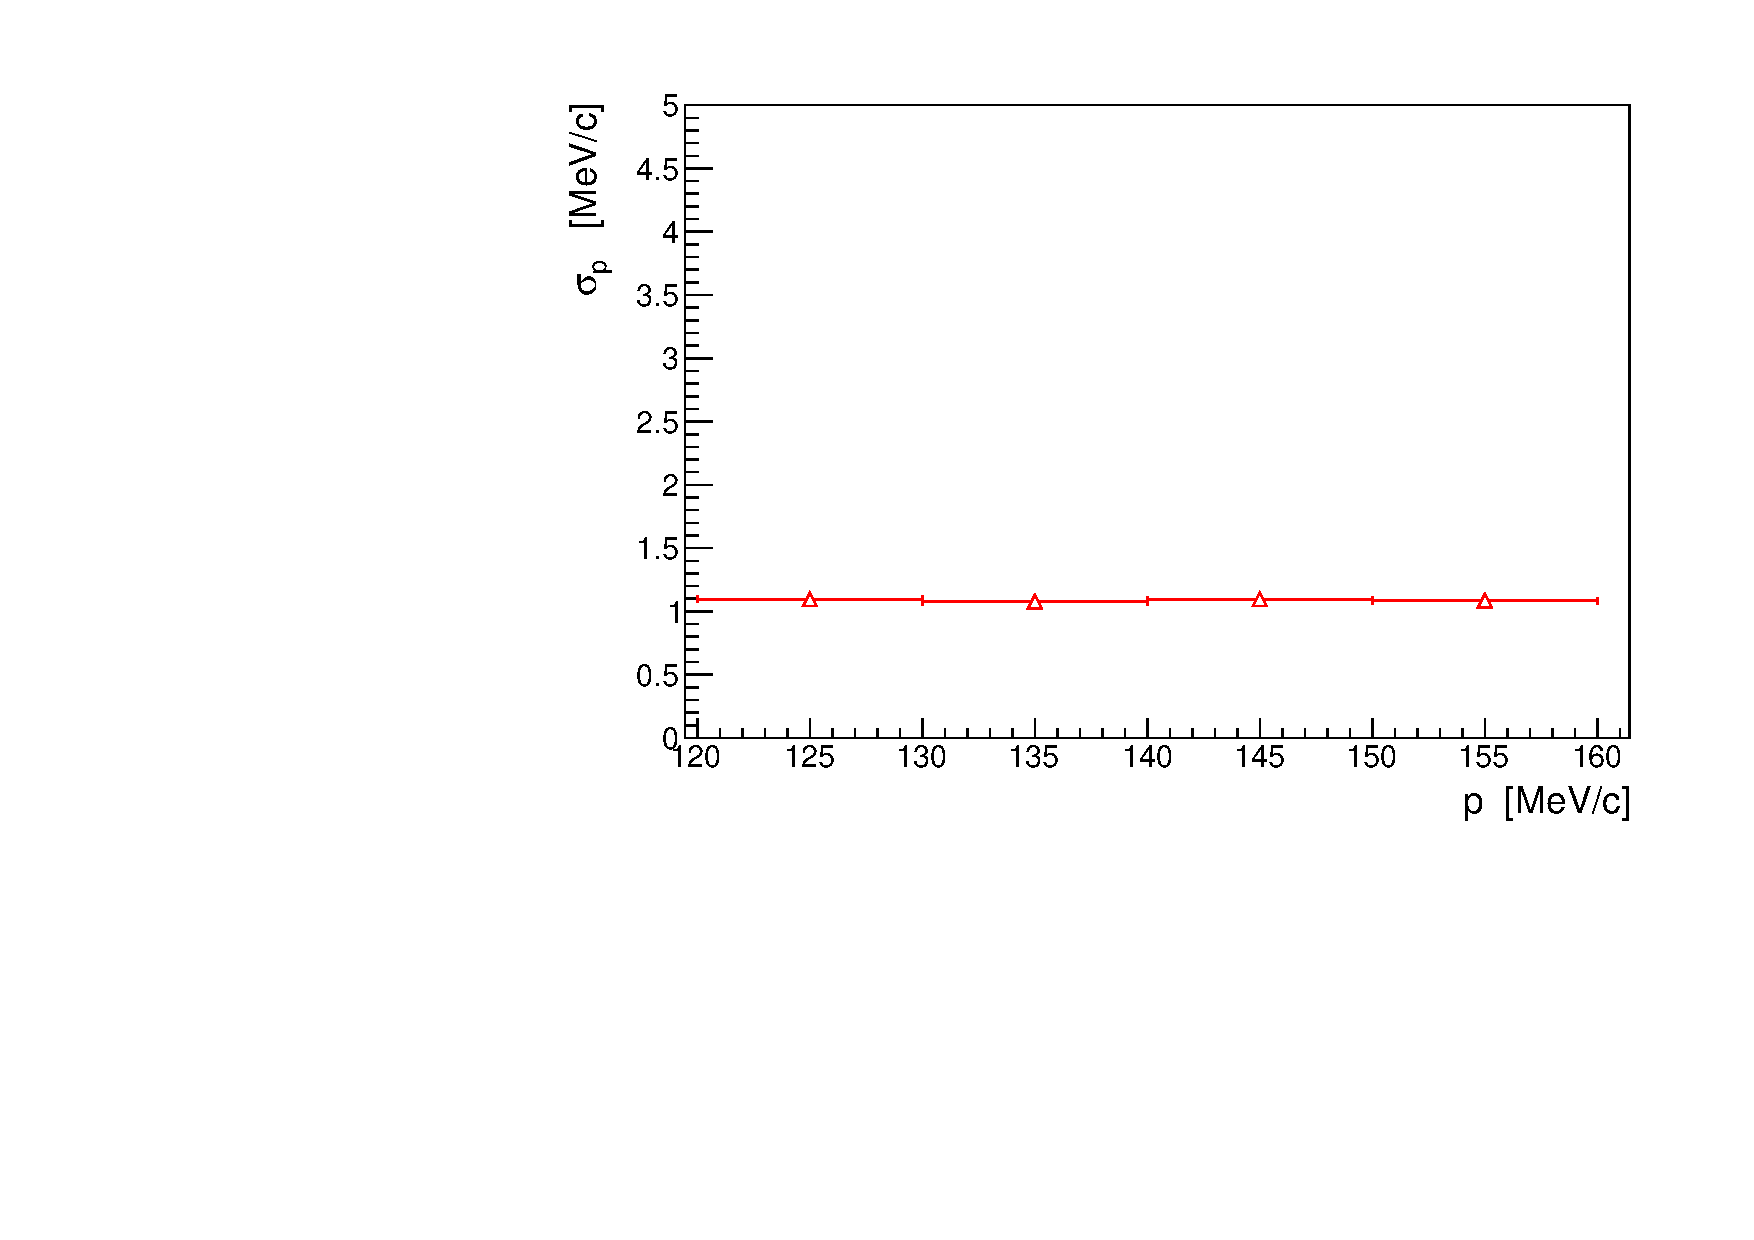
\includegraphics[width=0.5\textwidth]{upstream_p_resolution_p.pdf} \\
        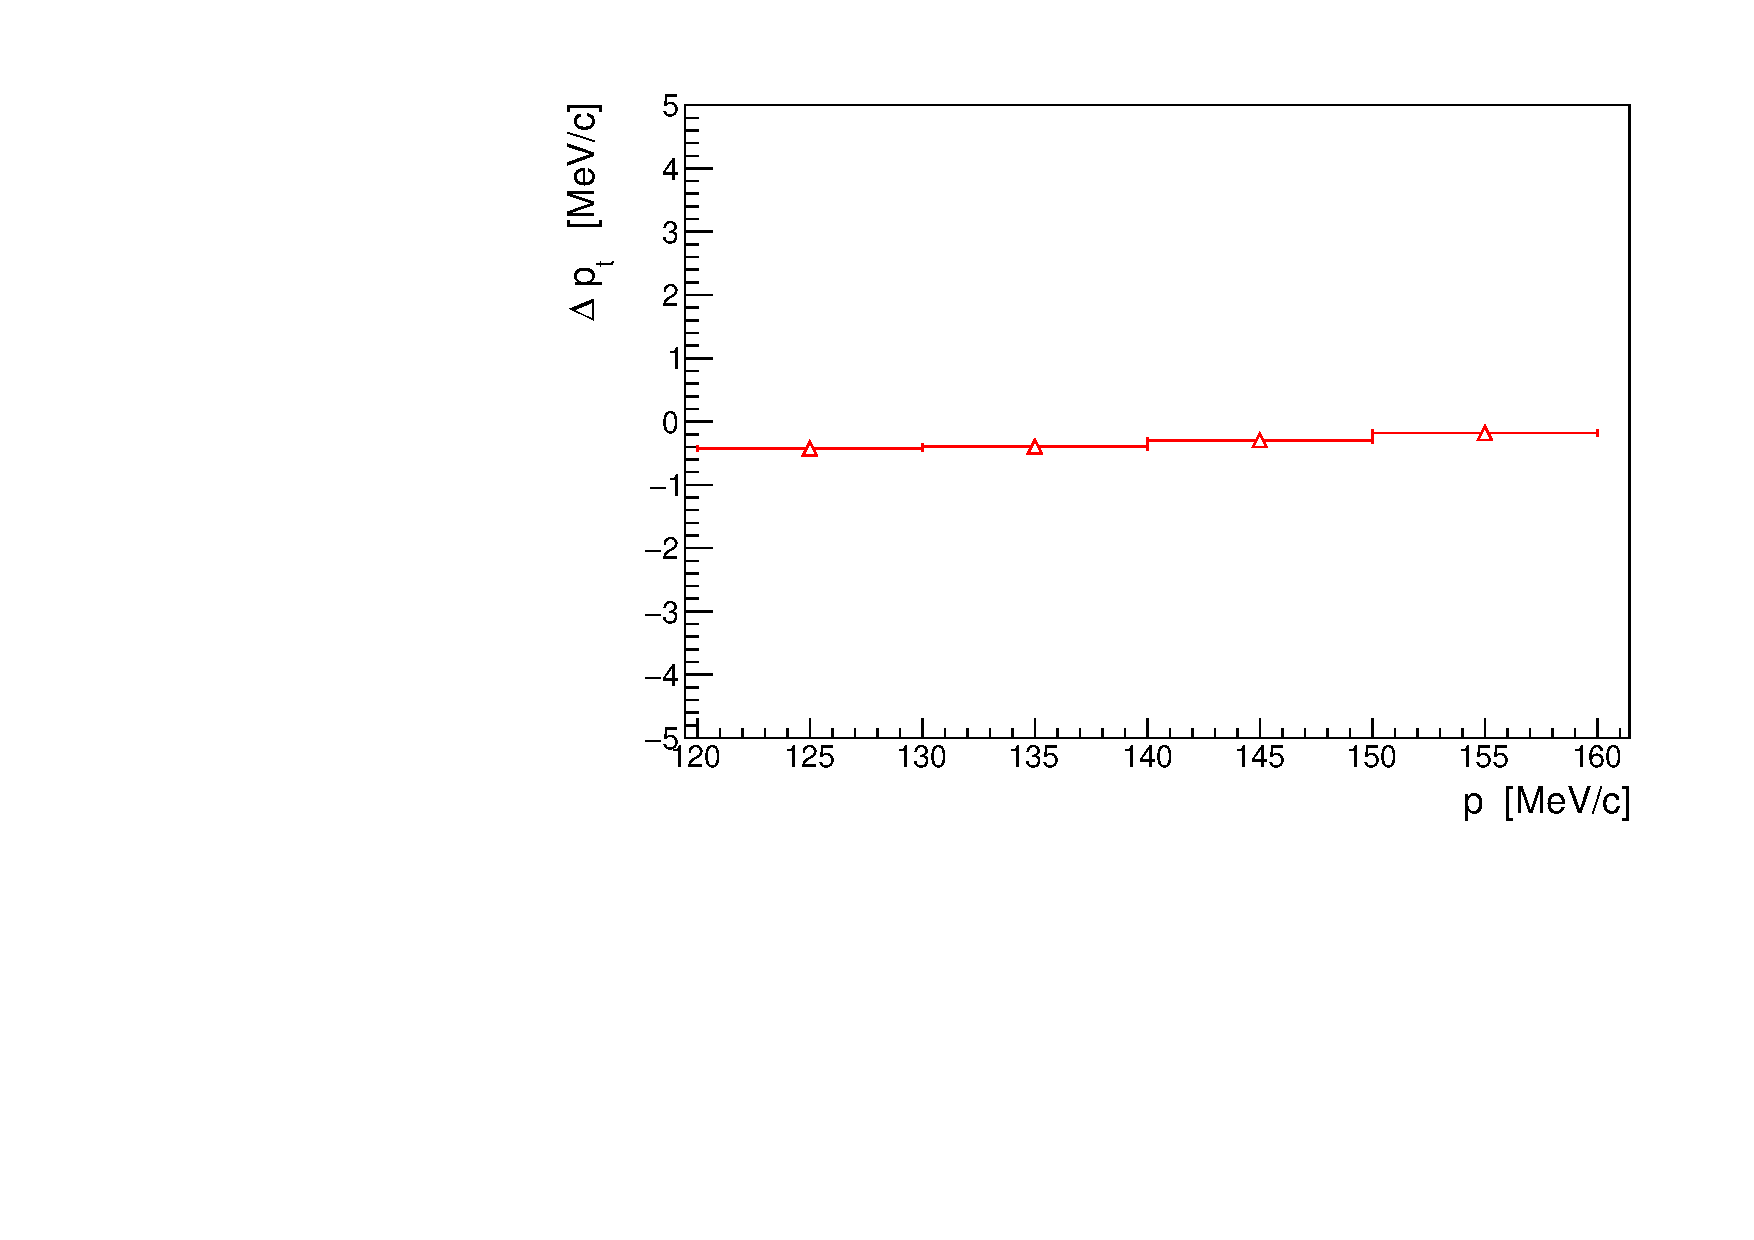
\includegraphics[width=0.5\textwidth]{upstream_pt_bias_p.pdf} &
        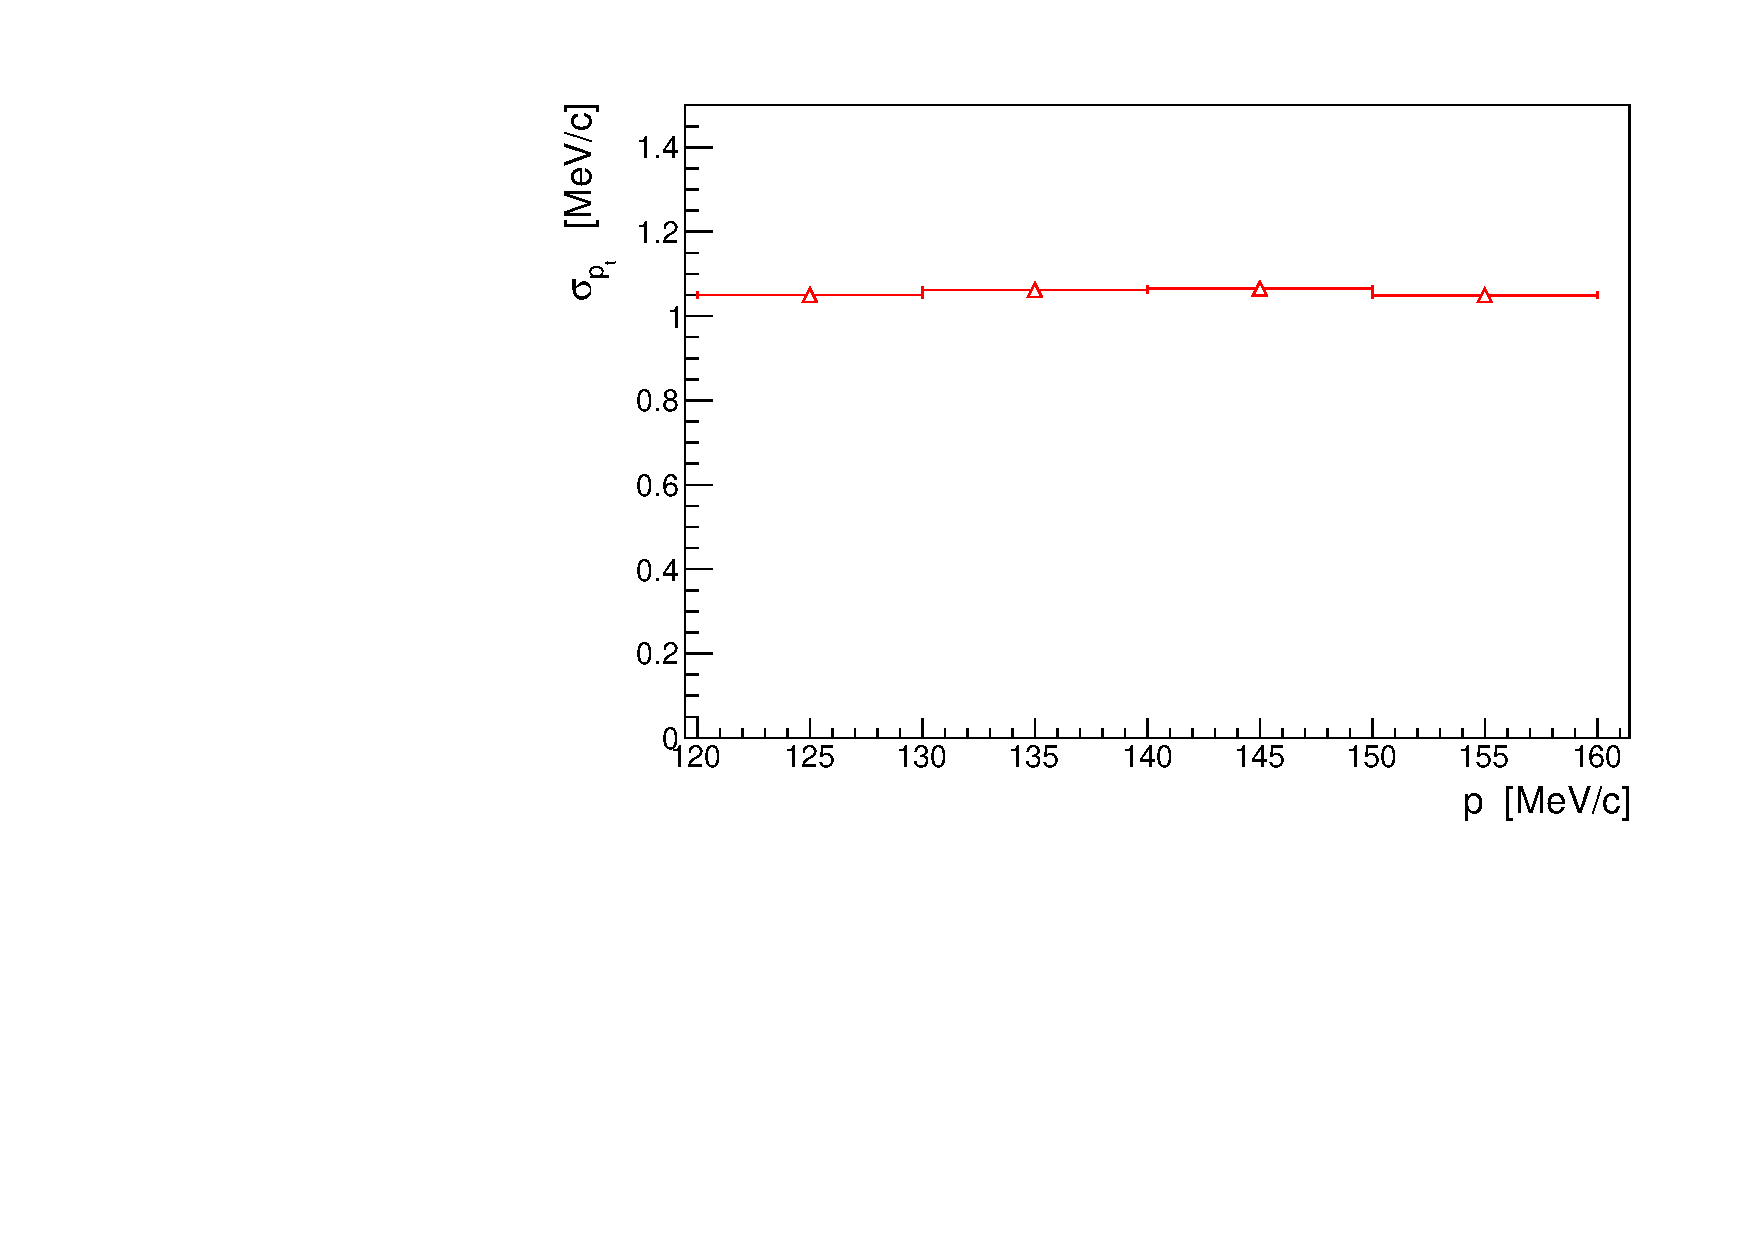
\includegraphics[width=0.5\textwidth]{upstream_pt_resolution_p.pdf}
    \end{tabular}
	\caption{\label{trackers:performance:resolutions:up}Predicted momentum reconstruction bias (left) and resolution (right) for the longitudinal (top) and transverse (bottom) momentum components in the upstream tracker.}
\end{figure}

\begin{figure}[ht]
	\centering
    \begin{tabular}{cc}
	    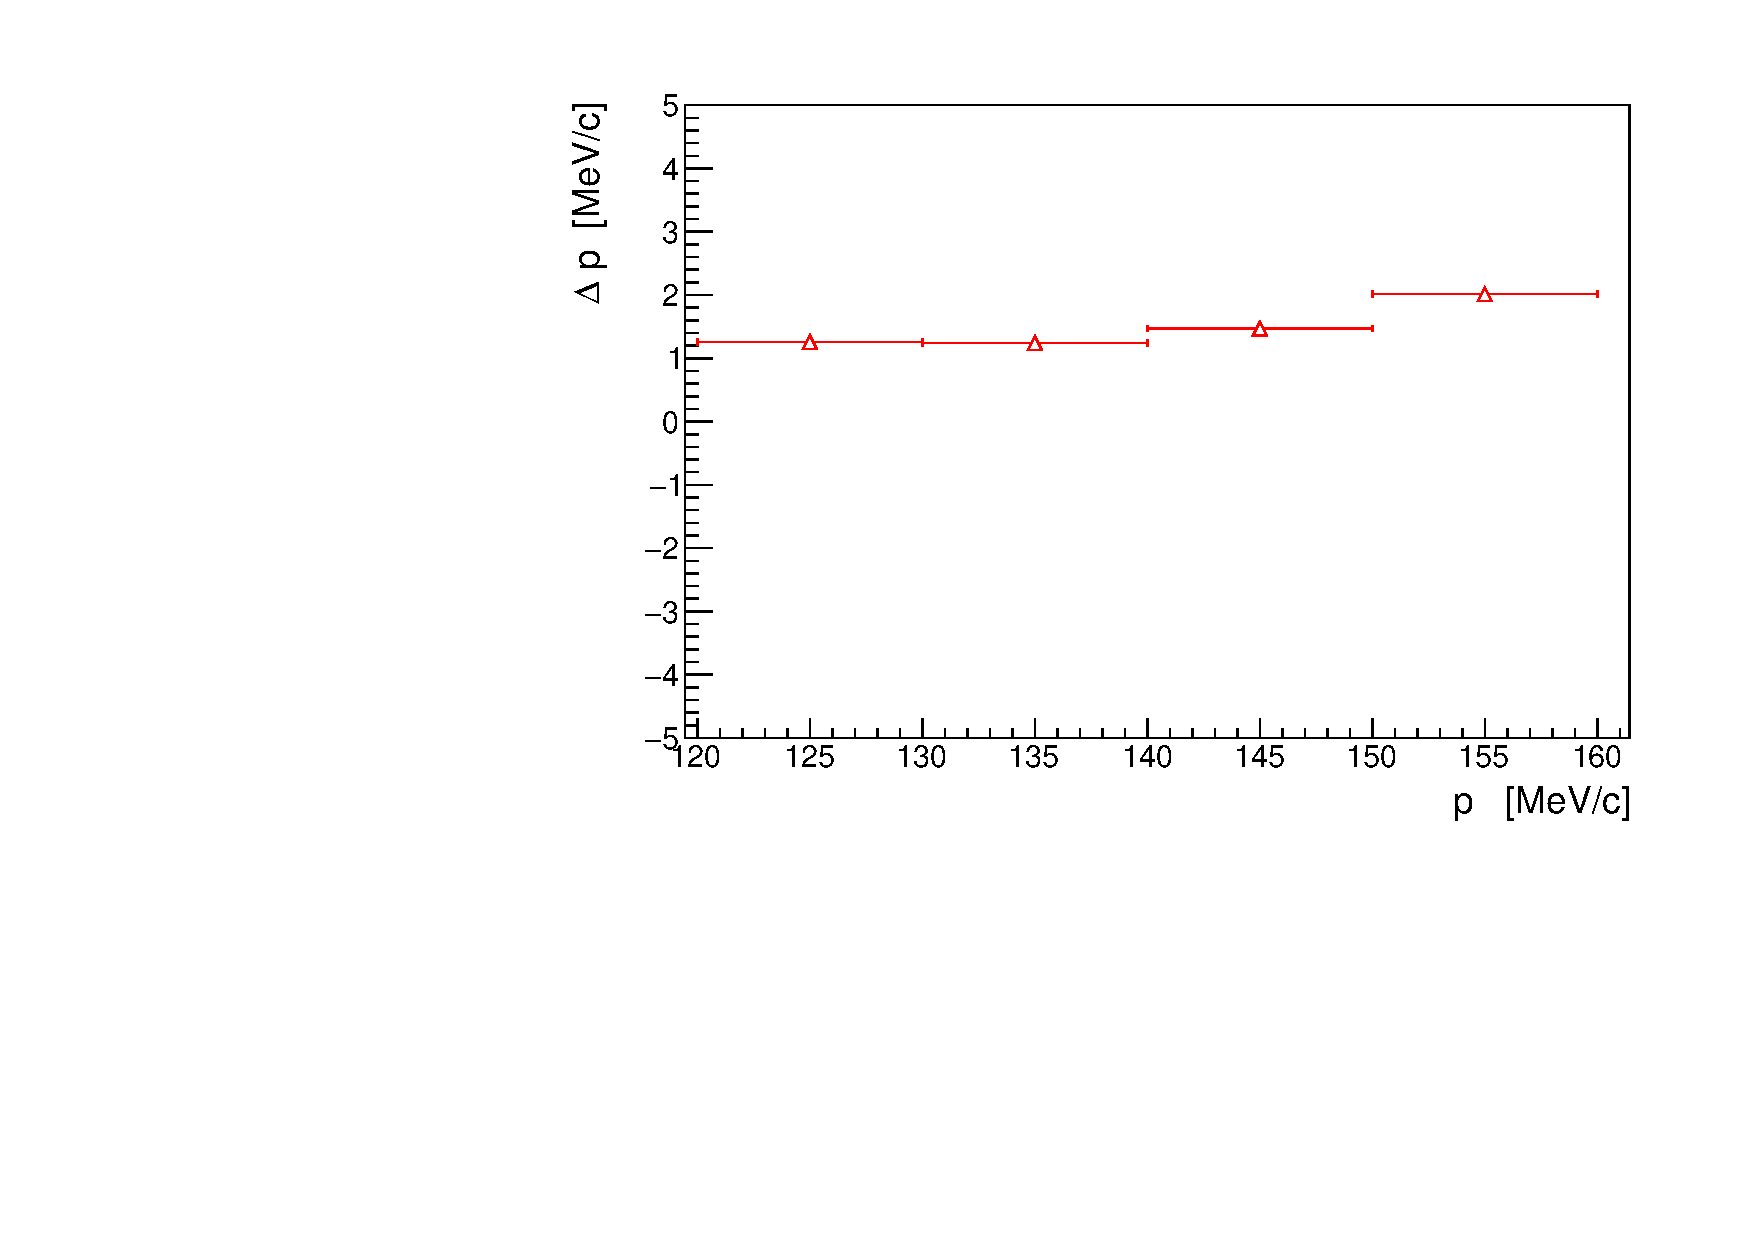
\includegraphics[width=0.5\textwidth]{downstream_p_bias_p.pdf} &	
        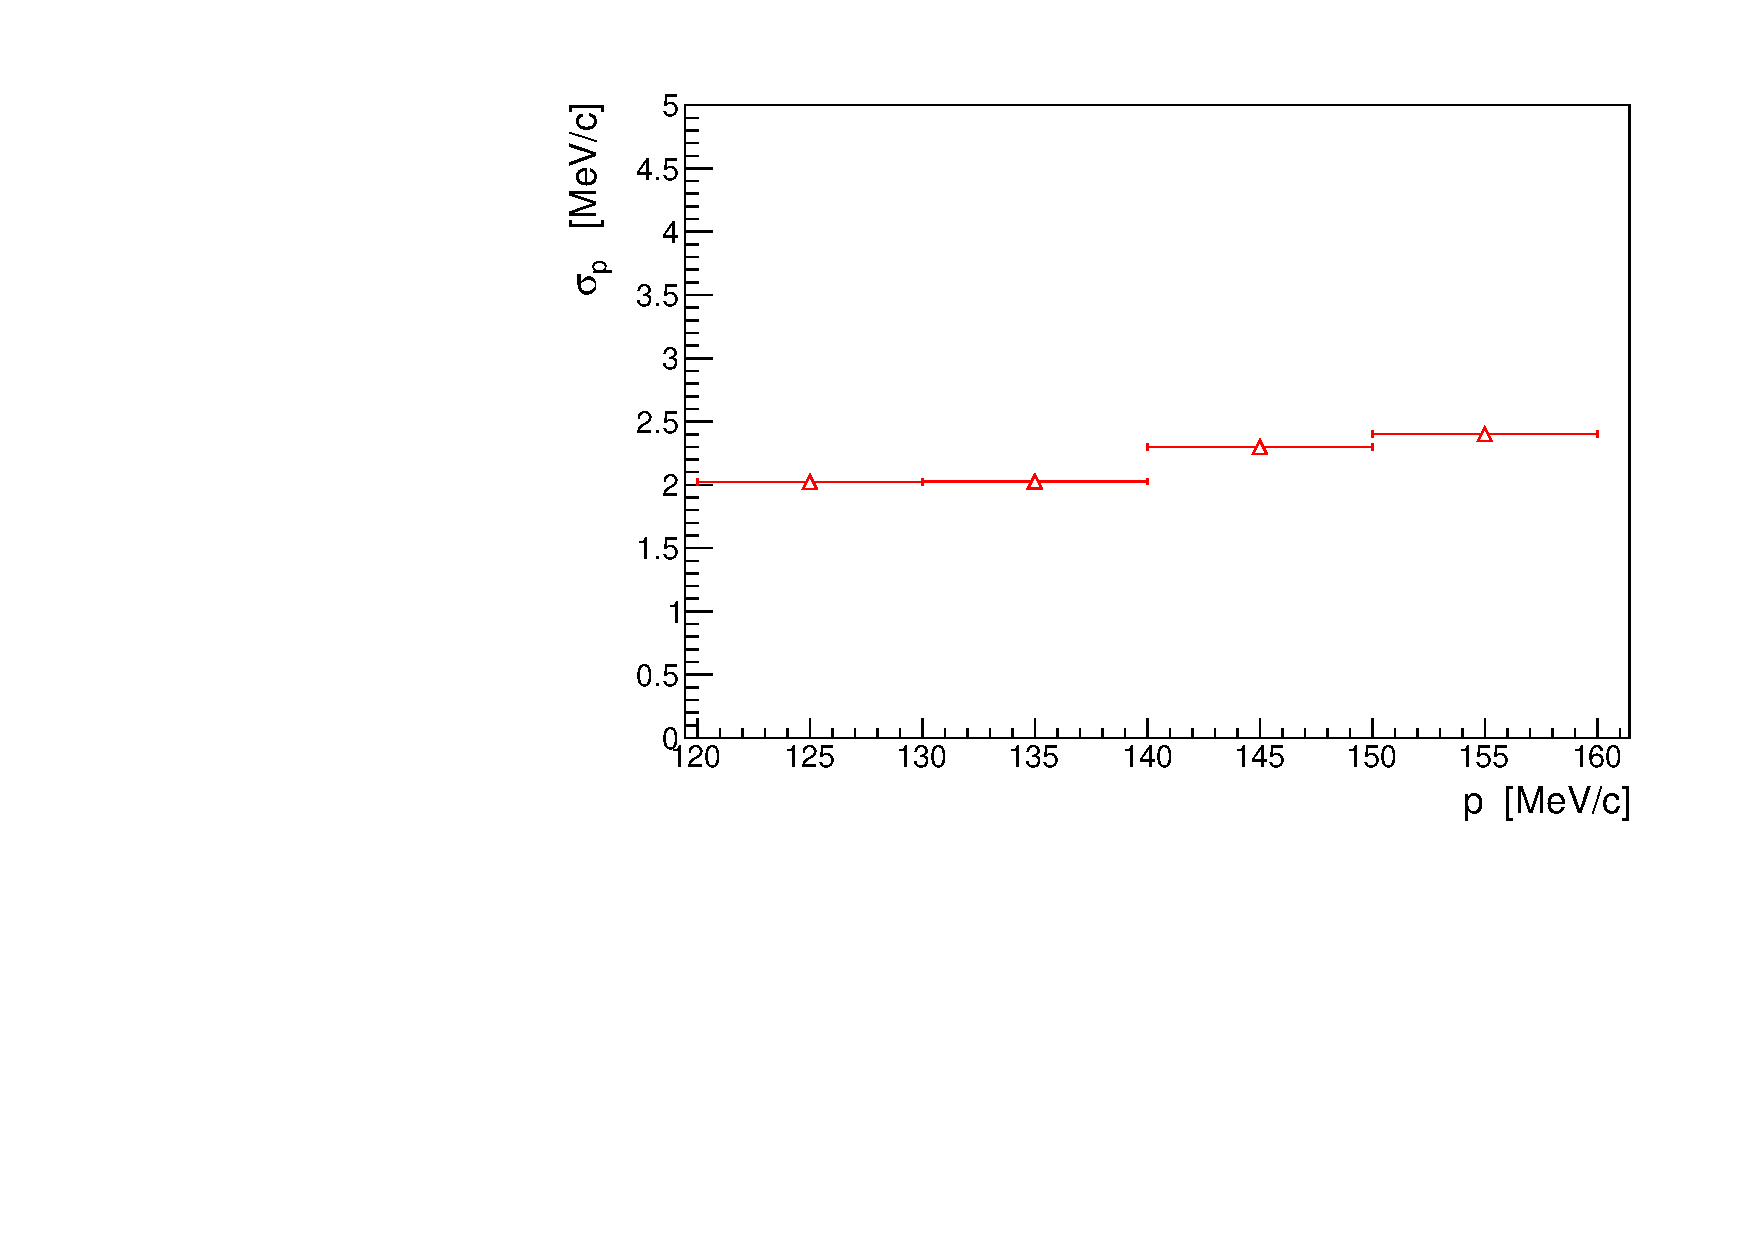
\includegraphics[width=0.5\textwidth]{downstream_p_resolution_p.pdf} \\
        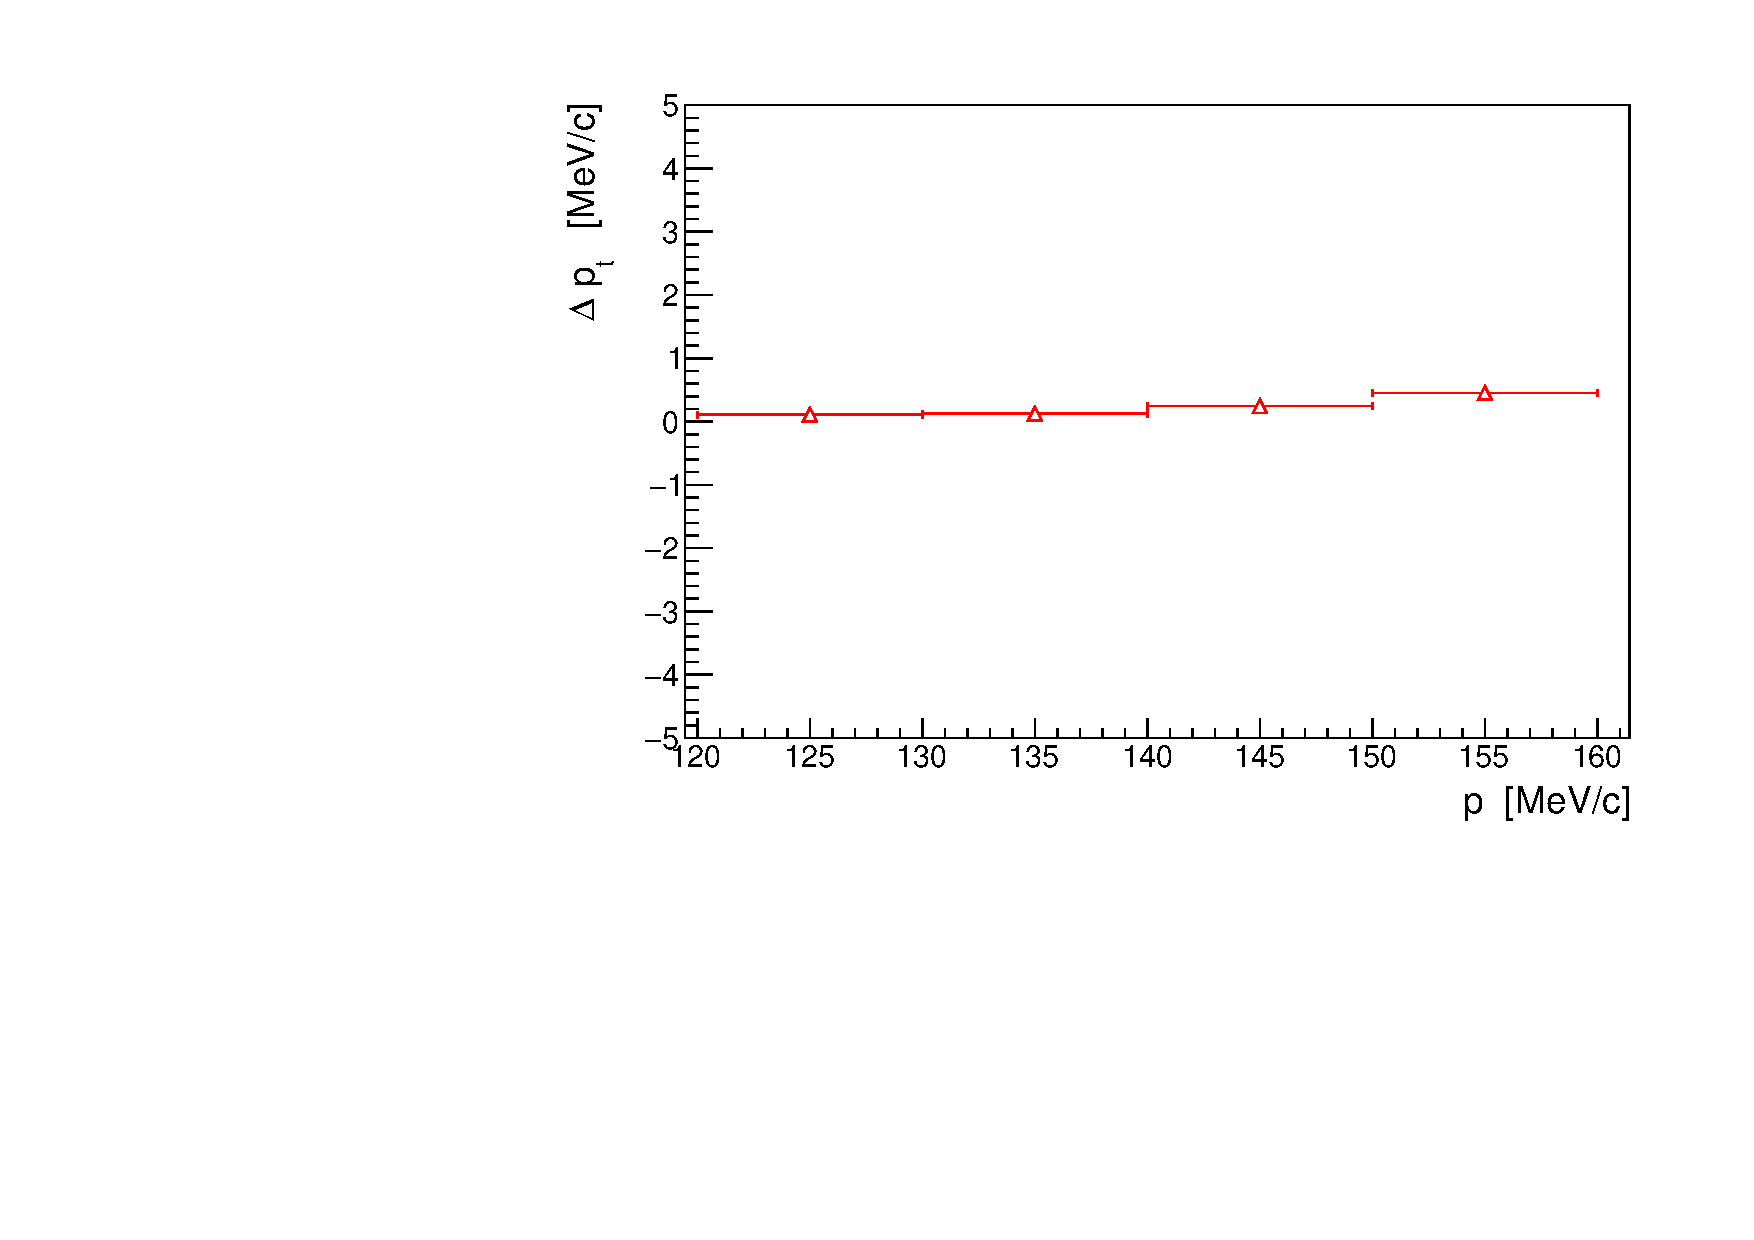
\includegraphics[width=0.5\textwidth]{downstream_pt_bias_p.pdf} &
        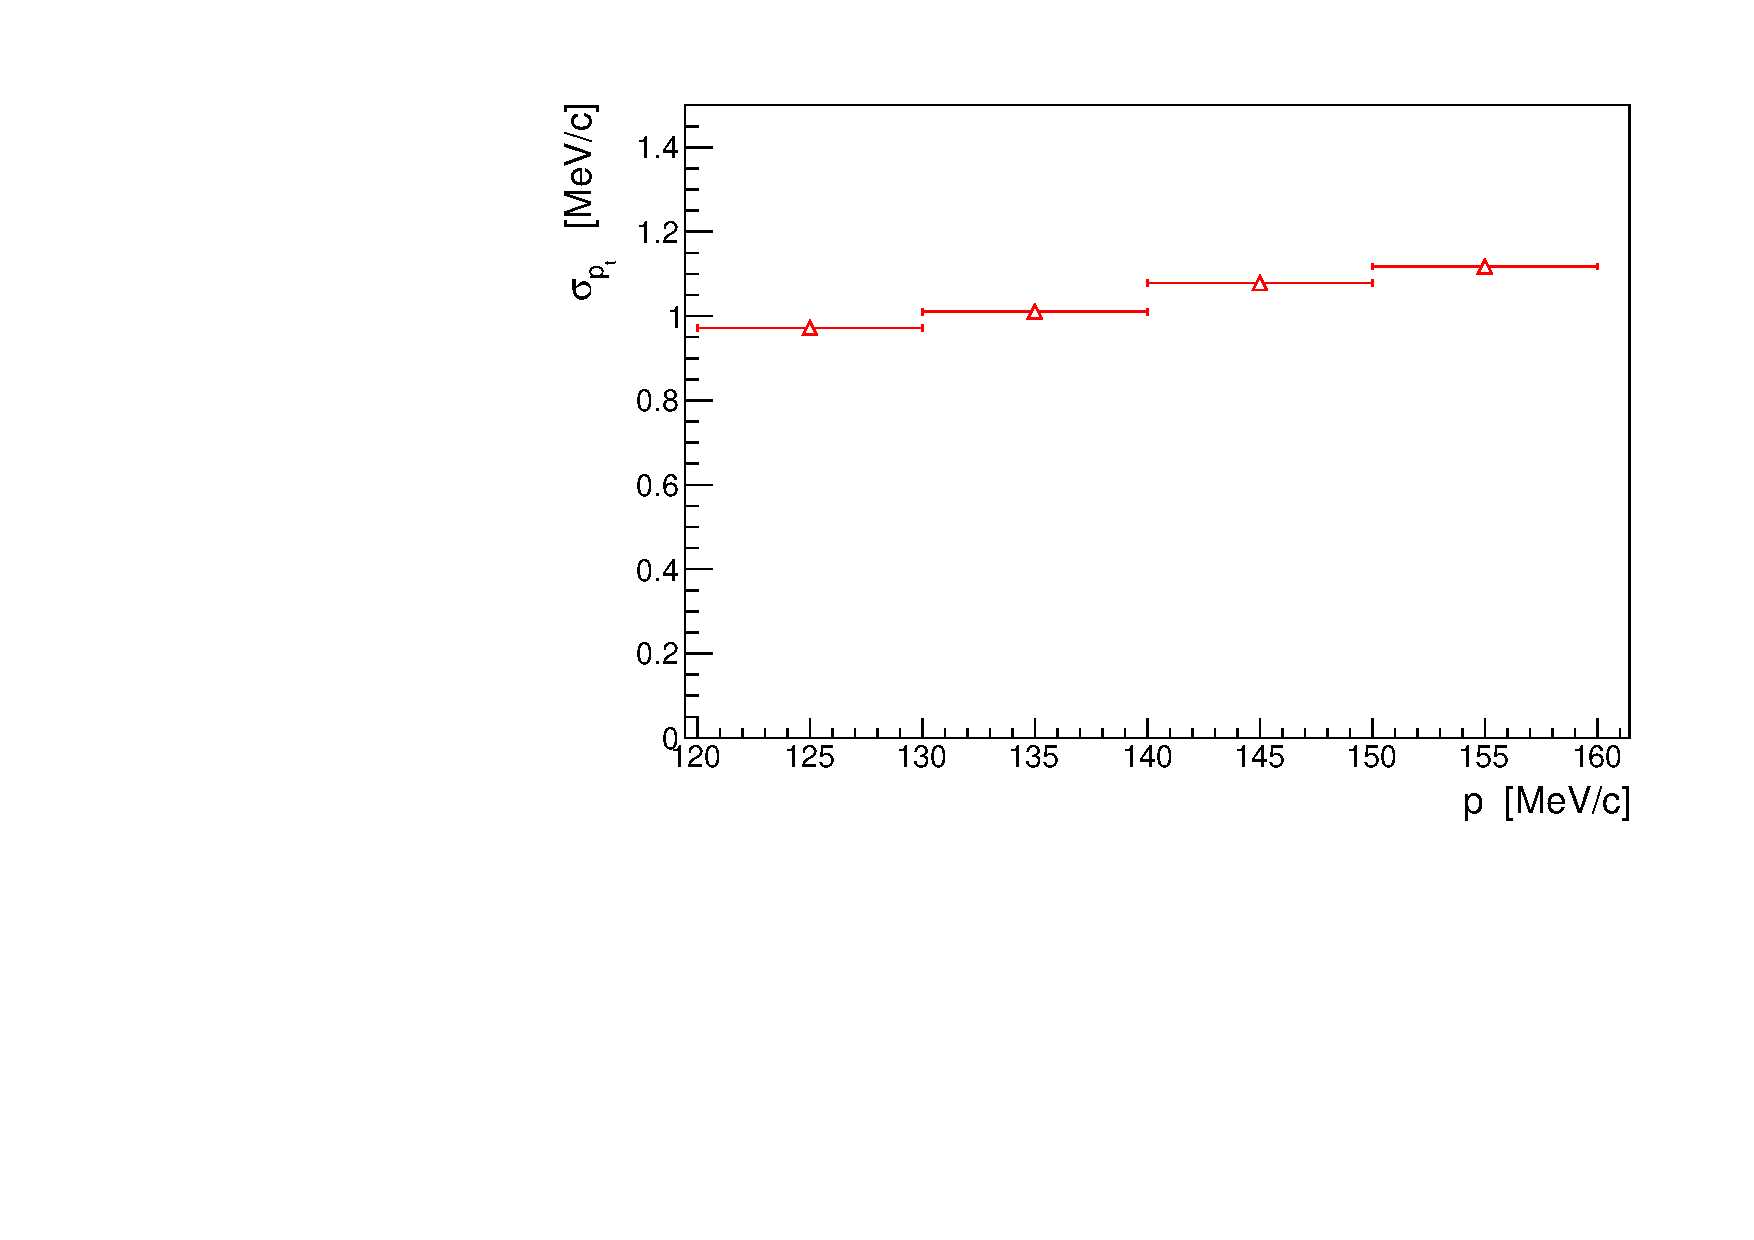
\includegraphics[width=0.5\textwidth]{downstream_pt_resolution_p.pdf}
    \end{tabular}
	\caption{\label{trackers:performance:resolutions:down}Predicted momentum reconstruction bias (left) and resolution (right) for the longitudinal (top) and transverse (bottom) momentum components in the downstream tracker.}
\end{figure}


\subsection{Tracker Efficiency Evolution}

Tracker efficiency with time (maybe 1 runs every 3 months since start shown?), 1/2 page, Paul K.
